\documentclass[10pt]{article}
\usepackage[utf8]{inputenc}
\usepackage[T1]{fontenc}
\usepackage{amsmath}
\usepackage{amsfonts}
\usepackage{amssymb}
\usepackage[version=4]{mhchem}
\usepackage{stmaryrd}
\usepackage{bbold}
\usepackage{graphicx}
\usepackage[export]{adjustbox}
\graphicspath{ {./images/} }

\title{Probability and Statistics - Elementary Probability Theory \\
 Joint Random Variables }

\author{Joint pmf/pdf\\
Independence \& Expectation\\
Conditional Distributions\\
Markov chains}
\date{}


\begin{document}
\maketitle


\section*{Joint Random Variables}
We often need to study the outcomes of multiple experiments or analyze multiple random variables for a given experiment, e.g.:

\begin{itemize}
  \item Two Dice: $X \in\{1, \ldots, 6\}, Y \in\{1, \ldots, 6\}$.
  \item Coin and Die: $X \in\{0,1\}$ (Heads/Tails), $Y \in\{1, \ldots, 6\}$.
  \item Darts: $X \in \mathbb{R}$ coordinate, $Y \in \mathbb{R}$ coordinate.
\end{itemize}

Probability tables and conditional probabilities can help us understand dependences between events.

How do generalize these ideas to random variables?

\section*{Definitions}
Suppose we have two random variables $X: S \rightarrow \mathbb{R}, Y: S \rightarrow \mathbb{R}$, where $S$ is the joint sample space.

If $X$ and $Y$ are instead defined on different experiments with sample spaces $S_{1}$ and $S_{2}$, we may set $S=S_{1} \times S_{2}$, or a subset thereof, consisting of pairs $s \equiv\left(s_{1}, s_{2}\right), s_{1} \in S_{1}, s_{2} \in S_{2}$.

As before, an event $E$ is a subset of outcomes $s \in S$ and has an associated probability measure $\mathrm{P}(E)$.

We may analyze joint r.vs. in terms of a random vector $Z=(X, Y): S \rightarrow \mathbb{R}^{2}$, i.e. a mapping $Z(s) \rightarrow(X(s), Y(s))$.

\section*{Induced probability}
\begin{itemize}
  \item For each pair $(x, y) \in \mathbb{R}^{2}$, let $S_{x y} \subseteq S$ be the set containing just those elements of $S$ which are mapped by $X$ to numbers no greater than $x$ and by $Y$ to numbers no greater than $y$, i.e.
\end{itemize}

$$
S_{x y}=\{s \in S \mid X(s) \leq x \text { and } Y(s) \leq y\}
$$

\begin{itemize}
  \item The induced probability will now be a function
\end{itemize}

$$
\mathrm{P}_{Z}(X \leq x, Y \leq y)=\mathrm{P}_{Z}((-\infty, x],(-\infty, y])=\mathrm{P}\left(S_{x y}\right)
$$

for $x, y \in \mathbb{R}$.

\section*{Joint Cumulative Distribution Function}
We can now define the joint cumulative distribution function (joint cdf) as

\section*{Definition}
$$
F(x, y)=\mathrm{P}_{Z}(X \leq x, Y \leq y), \quad x, y \in \mathbb{R}
$$

The marginal cdfs for $X$ and $Y$, i.e. the cdfs for $X$ and $Y$ alone can be easily recovered:

$$
\begin{array}{ll}
F_{X}(x)=F(x, \infty), & x \in \mathbb{R}, \\
F_{Y}(y)=F(\infty, y), & y \in \mathbb{R},
\end{array}
$$

i.e., $F_{X}(x)$ and $F_{Y}(y)$ are the cdfs for $X$ and $Y$ alone, irrespective of the value of the other r.v.

\section*{Properties of a Joint cdf}
For $F$ to be a valid joint cdf, the following conditions must hold:\\
(1) $0 \leq F(x, y) \leq 1, \forall x, y \in \mathbb{R}$;\\
(2) Monotonicity: $\forall x_{1}, x_{2}, y_{1}, y_{2} \in \mathbb{R}$,\\
$x_{1}<x_{2} \Rightarrow F\left(x_{1}, y_{1}\right) \leq F\left(x_{2}, y_{1}\right)$ and\\
$y_{1}<y_{2} \Rightarrow F\left(x_{1}, y_{1}\right) \leq F\left(x_{1}, y_{2}\right)$;\\
(3) $F(x,-\infty)=F(-\infty, y)=0$ and $F(\infty, \infty)=1 \quad \forall x, y \in \mathbb{R}$.

\section*{Interval Probabilities}
Suppose we are interested in whether the random variable pair $Z=(X, Y)$ lie in the interval cross product $\left(x_{1}, x_{2}\right] \times\left(y_{1}, y_{2}\right]$; that is, if $x_{1}<X \leq x_{2}$ and $y_{1}<Y \leq y_{2}$.\\
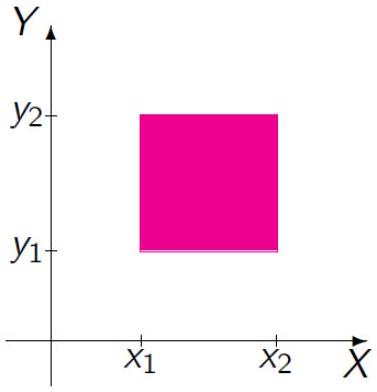
\includegraphics[max width=\textwidth, center]{2025_05_11_84d245f69223a25e0522g-07}

\begin{itemize}
  \item $\mathrm{P}_{Z}\left(x_{1}<X \leq x_{2}, Y \leq y\right)=F\left(x_{2}, y\right)-F\left(x_{1}, y\right)$
  \item Hence:
\end{itemize}

$$
\begin{gathered}
\mathrm{P}_{Z}\left(x_{1}<X \leq x_{2}, y_{1}<Y \leq y_{2}\right)= \\
F\left(x_{2}, y_{2}\right)-F\left(x_{1}, y_{2}\right)-F\left(x_{2}, y_{1}\right)+F\left(x_{1}, y_{1}\right)
\end{gathered}
$$

\section*{Joint pmf/pdf}
\section*{Joint Probability Mass Functions}
If $X$ and $Y$ are both discrete random variables, then we can define the joint probability mass function by\\
Definition

$$
p(x, y)=\mathrm{P}_{Z}(X=x, Y=y), \quad x, y \in \mathbb{R} .
$$

We can recover the marginal pmfs $p_{X}$ and $p_{Y}$ since $\forall x, y \in \mathbb{R}$

$$
p_{X}(x)=\sum_{y} p(x, y), \quad p_{Y}(y)=\sum_{x} p(x, y) .
$$

This may be seen as a consequence of the law of total probability.

\section*{Properties of a Joint pmf}
For $p$ to be a valid pmf, we need to make sure the following conditions hold.\\
(1) $0 \leq p(x, y) \leq 1, \forall x, y \in \mathbb{R}$;\\
(2) $\sum_{y} \sum_{x} p(x, y)=1$.

The previous definitions readily generalize to $n$ random variables.

\section*{Example: Multinomial distribution}
Consider a sequence of $n$ independent and identical experiments with $r$ possible outcomes, each with probability $q_{i}, \sum_{i=1}^{r} q_{i}=1$.\\
Let $X_{i}$ be the number of experiments that yield outcome $i$, then:

$$
p\left(n_{1}, \ldots, n_{r}\right)=\mathrm{P}_{Z}\left(X_{1}=n_{1}, \ldots, X_{r}=n_{r}\right)=\frac{n!}{n_{1}!n_{2}!\cdots n_{r}!} q_{1}^{n_{1}} q_{2}^{n_{2}} \cdots q_{r}^{n_{r}}
$$

This is due to independence, since a sequence has probability

$$
q_{1}^{n_{1}} q_{2}^{n_{2}} \cdots q_{r}^{n_{r}} \quad\left(n_{1}+n_{2}+\ldots+n_{r}=n\right)
$$

and the number of sequences that yield $\left(n_{1}, \ldots, n_{r}\right)$ is

$$
\binom{n}{n_{1}}\binom{n-n_{1}}{n_{2}} \cdots\binom{n-\sum_{i=1}^{r-1} n_{i}}{n_{r}}=\frac{n!}{n_{1}!n_{2}!\cdots n_{r}!}
$$

\section*{Example: Linearity of expectation}
We had seen that $E[X+Y]=E[X]+E[Y]$ also for dependent variables. We can now prove it using marginal pmfs.

$$
\begin{aligned}
E[X+Y] & =\sum_{x} \sum_{y}(x+y) p(x, y) \\
& =\sum_{x} \sum_{y} x p(x, y)+\sum_{x} \sum_{y} y p(x, y) \\
& =\sum_{x} x \sum_{y} p(x, y)+\sum_{y} y \sum_{x} p(x, y) \\
& =\sum_{x} x p_{X}(x)+\sum_{x} y p_{Y}(y) \\
& =E[X]+E[Y]
\end{aligned}
$$

The proof can be generalized to $n$ random variables and to the continuous case.

\section*{Joint Probability Density Functions}
In the continuous case, if $\exists f: \mathbb{R} \times \mathbb{R} \rightarrow \mathbb{R}$ s.t.

$$
F(x, y)=\int_{t=-\infty}^{y} \int_{s=-\infty}^{x} f(s, t) d s d t, \quad x, y \in \mathbb{R}
$$

then we say $X$ and $Y$ are jointly continuous and we refer to $f$ as the joint probability density function of $X$ and $Y$.

By the Fundamental Theorem of Calculus we then have

$$
f(x, y)=\frac{\partial^{2}}{\partial x \partial y} F(x, y)
$$

\section*{Properties of a Joint pdf}
For $f$ to be a valid pdf, we need to make sure the following conditions hold.\\
(1) $f(x, y) \geq 0, \forall x, y \in \mathbb{R}$;\\
(2) $\int_{y=-\infty}^{\infty} \int_{x=-\infty}^{\infty} f(x, y) d x d y=1$.

The previous definitions readily generalize using separate integrals for each random variable.

\section*{Marginal Density Functions}
The marginal pdfs $f_{X}$ and $f_{Y}$ are then derivatives of the joint cdf:

$$
\begin{aligned}
f_{X}(x) & =\frac{d}{d x} F_{X}(x)=\frac{d}{d x} F(x, \infty) \\
& =\frac{d}{d x} \int_{y=-\infty}^{\infty} \int_{s=-\infty}^{x} f(s, y) d s d y \\
f_{Y}(y) & =\frac{d}{d y} \int_{x=-\infty}^{\infty} \int_{s=-\infty}^{y} f(x, s) d s d x
\end{aligned}
$$

and applying again the Fundamental Theorem of Calculus

$$
\begin{aligned}
& f_{X}(x)=\int_{y=-\infty}^{\infty} f(x, y) d y \\
& f_{Y}(y)=\int_{x=-\infty}^{\infty} f(x, y) d x
\end{aligned}
$$

\section*{Q\&A: Marginal pdf}
Suppose continuous r.vs. $(X, Y) \in \mathbb{R}^{2}$ have joint pdf

$$
f(x, y)= \begin{cases}1, & |x|+|y|<1 / \sqrt{2} \\ 0, & \text { otherwise } .\end{cases}
$$

Q: Determine the marginal pdfs for $X$ and $Y$.

\section*{Independence \& Expectation}
\section*{Independence of Random Variables}
Two random variables $X$ and $Y$ are independent if and only if

$$
F(x, y)=F_{X}(x) F_{Y}(y), \quad \forall x, y
$$

Equivalently, this property specializes as follows:

\begin{itemize}
  \item Discrete case: independence holds if and only if
\end{itemize}

$$
p(x, y)=p_{X}(x) p_{Y}(y), \quad \forall x, y
$$

\begin{itemize}
  \item Continuous case: independence holds if and only if
\end{itemize}

$$
f(x, y)=f_{X}(x) f_{Y}(y), \quad \forall x, y
$$

\section*{Q\&A: Marginal pdf - continued}
Consider again $(X, Y) \in \mathbb{R}^{2}$ with joint pdf

$$
f(x, y)= \begin{cases}1, & |x|+|y|<1 / \sqrt{2} \\ 0, & \text { otherwise } .\end{cases}
$$

Q: are $X$ and $Y$ independent?

\section*{Example: Independent random variables}
Suppose that the lifetime, $X$, and brightness, $Y$ of a light bulb are modelled as continuous random variables. Let their joint pdf be

$$
f(x, y)=\lambda_{1} \lambda_{2} e^{-\lambda_{1} x-\lambda_{2} y}, \quad x, y>0 .
$$

Are lifetime and brightness independent?\\
Solution:

\begin{itemize}
  \item The marginal pdf for $X$ is
\end{itemize}

$$
\begin{aligned}
f(x) & =\int_{y=-\infty}^{\infty} f(x, y) d y=\int_{y=0}^{\infty} \lambda_{1} \lambda_{2} e^{-\lambda_{1} x-\lambda_{2} y} d y \\
& =\lambda_{1} e^{-\lambda_{1} x}
\end{aligned}
$$

\begin{itemize}
  \item Similarly $f(y)=\lambda_{2} e^{-\lambda_{2} y}$. Hence $f(x, y)=f(x) f(y)$ and $X$ and $Y$ are independent.
\end{itemize}

\section*{Expectation of a function of r.vs: $\mathrm{E}(g(X, Y))$}
Let $g$ be a bivariate function of the random variables $X$ and $Y$, defined by $g: \mathbb{R} \times \mathbb{R} \rightarrow \mathbb{R}$.

\begin{itemize}
  \item If $X$ and $Y$ are discrete, we define $\mathrm{E}(g(X, Y))$ by
\end{itemize}

\section*{Definition}
$$
\mathrm{E}(g(X, Y))=\sum_{y} \sum_{x} g(x, y) p(x, y) .
$$

\begin{itemize}
  \item If $X$ and $Y$ are jointly continuous, we define $\mathrm{E}(g(X, Y))$ by Definition
\end{itemize}

$$
\mathrm{E}(g(X, Y))=\int_{y=-\infty}^{\infty} \int_{x=-\infty}^{\infty} g(x, y) f(x, y) d x d y
$$

Immediately from these definitions we have the following:

\begin{itemize}
  \item If $g(X, Y)=g_{1}(X)+g_{2}(Y)$,
\end{itemize}

$$
\mathrm{E}\left(g_{1}(X)+g_{2}(Y)\right)=E_{X}\left(g_{1}(X)\right)+E_{Y}\left(g_{2}(Y)\right) .
$$

\begin{itemize}
  \item If $g(X, Y)=g_{1}(X) g_{2}(Y)$ and $X$ and $Y$ are independent,
\end{itemize}

$$
\mathrm{E}\left(g_{1}(X) g_{2}(Y)\right)=\mathrm{E}_{X}\left(g_{1}(X)\right) \mathrm{E}_{Y}\left(g_{2}(Y)\right) .
$$

\begin{itemize}
  \item In particular, considering $g(X, Y)=X Y$ for independent $X, Y$ we have
\end{itemize}

$$
\mathrm{E}(X Y)=\mathrm{E}_{X}(X) \mathrm{E}_{Y}(Y) .
$$

\section*{Covariance}
\begin{itemize}
  \item For a single r.v. $X$ we considered the expectation of $g(X)=\left(X-\mu_{X}\right)\left(X-\mu_{X}\right)$, i.e., the variance and denoted $\sigma_{X}^{2}$.
  \item The bivariate extension of this is the expectation of $g(X, Y)=\left(X-\mu_{X}\right)\left(Y-\mu_{Y}\right)$.
  \item We define the covariance of $X$ and $Y$ by
\end{itemize}

$$
\begin{aligned}
\sigma_{X Y}=\operatorname{Cov}(X, Y) & =\mathrm{E}\left[\left(X-\mu_{X}\right)\left(Y-\mu_{Y}\right)\right] \\
& =\mathrm{E}[X Y]-\mu_{X} \mu_{Y}
\end{aligned}
$$

\begin{itemize}
  \item For independent r.vs., $\mathrm{E}[X Y]=\mathrm{E}_{X}[X] \mathrm{E}_{Y}[Y]$ so $\sigma_{X Y}=0$.
\end{itemize}

\section*{Correlation}
\begin{itemize}
  \item Covariance measures how two random variables change in tandem with one another, and so is closely related to the idea of correlation.
  \item The correlation of $X$ and $Y$ is defined by
\end{itemize}

$$
\rho_{X Y}=\operatorname{Cor}(X, Y)=\frac{\sigma_{X Y}}{\sigma_{X} \sigma_{Y}} .
$$

\begin{itemize}
  \item Unlike the covariance, correlation is invariant to the scale of the r.vs. $X$ and $Y$.
  \item It is easily shown that if $X$ and $Y$ are independent random variables, then $\sigma_{X Y}=\rho_{X Y}=0$.
\end{itemize}

\section*{Multivariate Normal distribution}
A random vector $X=\left(X_{1}, \ldots, X_{n}\right)$ with means $\mu=\left(\mu_{1}, \ldots, \mu_{n}\right)$ that has joint pdf

$$
f_{X}=\frac{1}{\sqrt{(2 \pi)^{n} \operatorname{det} \Sigma}} \exp \left(-\frac{1}{2}(x-\mu)^{T} \Sigma^{-1}(x-\mu)\right)
$$

is said to have a multivariate Normal distribution, where\\
$\mu=\left(\mu_{1}, \ldots, \mu_{n}\right)$ is the vector of means of $X_{1}, \ldots, X_{n}$\\
and the covariance matrix $\Sigma=\left[\operatorname{Cov}\left(X_{i}, X_{j}\right) ; 1 \leq i, j \leq n\right]$, which must be positive definite for a pdf to exist.

Note that the r.vs. $X_{1}, \ldots, X_{n}$ need not be independent.

\section*{Example: Independent normal r.vs.}
$$
\mu=(1,1), \operatorname{Var}\left(X_{1}\right)=\operatorname{Var}\left(X_{2}\right)=1, \operatorname{Cov}\left(X_{1}, X_{2}\right)=\operatorname{Cov}\left(X_{2}, X_{1}\right)=0
$$

\begin{center}
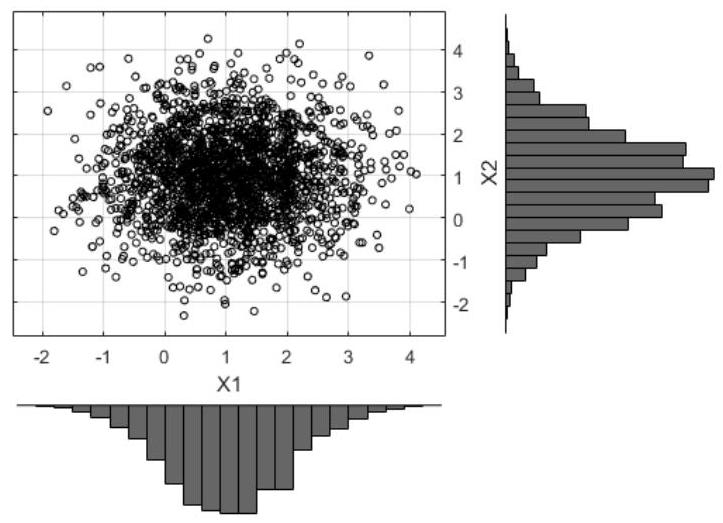
\includegraphics[max width=\textwidth]{2025_05_11_84d245f69223a25e0522g-26}
\end{center}

\section*{Example: Dependent normal r.vs.}
$$
\mu=(1,1), \operatorname{Var}\left(X_{1}\right)=\operatorname{Var}\left(X_{2}\right)=1, \operatorname{Cov}\left(X_{1}, X_{2}\right)=\operatorname{Cov}\left(X_{2}, X_{1}\right)=0.9
$$

\begin{center}
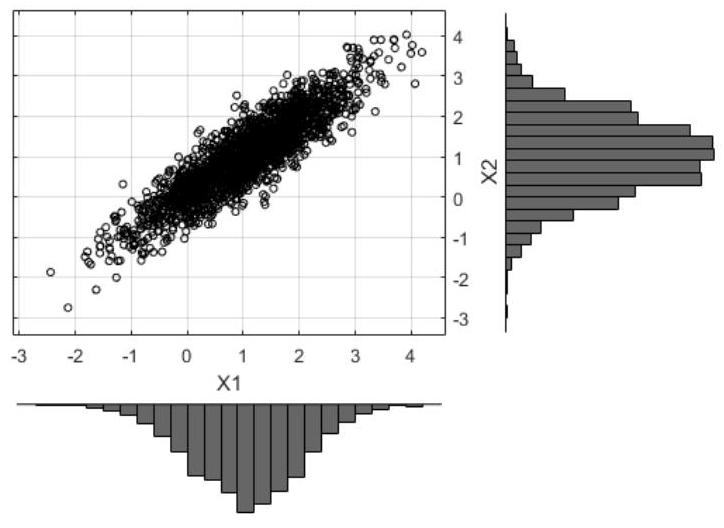
\includegraphics[max width=\textwidth]{2025_05_11_84d245f69223a25e0522g-27}
\end{center}

\section*{Conditional Distributions}
\section*{Conditional pmf}
We now extend the notion of conditional probability to r.vs.\\
For discrete r.vs. $X, Y$, we may define the conditional probability mass function as

$$
p_{X \mid Y}(x \mid y)=\frac{p(x, y)}{p_{Y}(y)}, \quad x, y \in \mathbb{R}
$$

which is valid for any $p_{Y}(y)>0$,\\
Bayes theorem may now be recast as

$$
p_{X \mid Y}(x \mid y)=\frac{p_{Y \mid X}(y \mid x) p_{X}(x)}{p_{Y}(y)}
$$

\section*{Conditional pdf}
For continuous r.vs., if $f_{X}(x)>0$ we set

$$
f_{Y \mid X}(y \mid x)=\frac{f(x, y)}{f_{X}(x)}, \quad x, y \in \mathbb{R}
$$

$X$ and $Y$ are now independent if and only if

$$
f_{Y \mid X}(y \mid x)=f_{Y}(y), \forall x, y \in \mathbb{R}
$$

Bayes theorem may now be rewritten as

$$
f_{X \mid Y}(x \mid y)=\frac{f_{Y \mid X}(y \mid x) f_{X}(x)}{f_{Y}(y)}
$$

\section*{Conditional cdfs}
Conditional cdfs and conditional pdfs/pmfs are related as follows:

\begin{itemize}
  \item For discrete random variables
\end{itemize}

$$
F_{X \mid Y}(x \mid y)=P(X \leq x \mid Y=y)=\sum_{u=-\infty}^{x} p_{X \mid Y}(u \mid y) .
$$

\begin{itemize}
  \item For continuous random variables
\end{itemize}

$$
F_{X \mid Y}(x \mid y)=P(X \leq x \mid Y=y)=\int_{u=-\infty}^{x} f_{X \mid Y}(u \mid y) d u
$$

\begin{itemize}
  \item Conditional interval probabilities follow from the conditional cdf
\end{itemize}

$$
P(a<X \leq b \mid Y=y)=F_{X \mid Y}(b \mid y)-F_{X \mid Y}(a \mid y)
$$

\section*{The Law of Total Probability for Joint RVs}
Corresponding to computing marginal from joint probabilities:

\begin{itemize}
  \item For discrete random variables
\end{itemize}

$$
p_{X}(x)=\sum_{y} p_{X \mid Y}(x \mid y) p_{Y}(y) .
$$

\begin{itemize}
  \item For continuous random variables
\end{itemize}

$$
f_{X}(x)=\int_{y=-\infty}^{\infty} f_{X \mid Y}(x \mid y) f_{Y}(y) d y
$$

Equivalently, $F_{X}(x)=\int_{y=-\infty}^{\infty} F_{X \mid Y}(x \mid y) f_{Y}(y) d y$.

\section*{Example: $\mathrm{P}(X<Y)$}
Let $X, Y$ be independent exponential random variables with parameters $\lambda, \mu$ respectively. What is the probability that $X<Y$ ?

Solution 1: The first way to solve this is directly:

$$
\begin{aligned}
\mathrm{P}(X<Y) & =\int_{x<y} f(x, y) \mathrm{d} x \mathrm{~d} y=\int_{y=-\infty}^{\infty} \int_{x=-\infty}^{y} f(x, y) \mathrm{d} x \mathrm{~d} y \\
& =\int_{y=-\infty}^{\infty} \int_{x=-\infty}^{y} f_{X}(x) f_{Y}(y) \mathrm{d} x \mathrm{~d} y \quad \text { (by independence) } \\
& =\int_{y=-\infty}^{\infty} F_{X}(y) f_{Y}(y) \mathrm{d} y=\int_{0}^{\infty}\left(1-e^{-\lambda y}\right) \mu e^{-\mu y} \mathrm{~d} y \\
& =1-\frac{\mu}{\lambda+\mu}=\frac{\lambda}{\lambda+\mu}
\end{aligned}
$$

\section*{Example: $\mathrm{P}(X<Y)$ with conditional probabilities}
Solution 2: The second way is more intuitive to some:

$$
\begin{aligned}
\mathrm{P}(X<Y) & =\int_{y=-\infty}^{\infty} \int_{X=-\infty}^{y} f(x, y) \mathrm{d} x \mathrm{~d} y \\
& =\int_{y=-\infty}^{\infty} \int_{X=-\infty}^{y} f_{X \mid Y}(x \mid y) f_{Y}(y) \mathrm{d} x \mathrm{~d} y \\
& =\int_{y=-\infty}^{\infty} F_{X \mid Y}(y \mid y) f_{Y}(y) \mathrm{d} y \\
& =\int_{0}^{\infty}\left(1-e^{-\lambda y}\right) \mu e^{-\mu y} \mathrm{~d} y \text { (by independence) } \\
& =1-\frac{\mu}{\lambda+\mu}=\frac{\lambda}{\lambda+\mu} .
\end{aligned}
$$

\section*{Conditional Expectation: $\mathrm{E}_{Y \mid X}(Y \mid x)$}
\begin{itemize}
  \item For discrete random variables, the conditional expectation of $Y$ given that $X=x$ is:
\end{itemize}

$$
E_{Y \mid X}(Y \mid x)=\sum_{y} y p_{Y \mid X}(y \mid x)
$$

\begin{itemize}
  \item Similarly, for continuous random variables
\end{itemize}

$$
\mathrm{E}_{Y \mid X}(Y \mid x)=\int_{y=-\infty}^{\infty} y f_{Y \mid X}(y \mid x) d y
$$

\begin{itemize}
  \item In either case, the conditional expectation is a function of $x$ but not of the random variable $Y$.
\end{itemize}

\section*{Law of total expectation}
\begin{itemize}
  \item We can define the random variable
\end{itemize}

$$
W=\mathrm{E}_{Y \mid X}(Y \mid X)
$$

as a function of the r.v. $X: S \rightarrow \mathbb{R}$ by $W(s)=\mathrm{E}_{Y \mid X}(Y \mid x)$, where $X(s)=x$.

\begin{itemize}
  \item Then we have
\end{itemize}

$$
\mathrm{E}_{Y}(Y)=\mathrm{E}_{X}\left(\mathrm{E}_{Y \mid X}(Y \mid X)\right)
$$

Holds for both discrete and continuous random variables. E.g. in the continuous case, the RHS gives

$$
\int_{x} \int_{y} y f_{Y \mid X}(y \mid x) f_{X}(x) \mathrm{d} y \mathrm{~d} x=\int_{y} \int_{x} y f(x, y) \mathrm{d} x \mathrm{~d} y=\int_{y} y f_{Y}(y) \mathrm{d} y
$$



\section*{Markov chains}
\section*{Discrete-Time Markov chain (DTMC)}
We learned to see a coin tossing sequence as a realization

$$
0,1,0,1,0,1,1,0,1, \ldots
$$

of i.i.d. r.vs. $X_{0}, X_{1}, \ldots$, taking values in $J=\operatorname{supp}\left(X_{i}\right)=\{0,1\}$.\\
DTMCs generalize this to arbitrary support and dependent r.vs:

\begin{itemize}
  \item $J$ is called the state space, its elements are the states $j \in J$.
  \item $X_{n}, n \geq 0$, takes values in $J$ and models the state at time $n$.
  \item A realization of $X_{0}, X_{1}, \ldots$, is called a sample path.
\end{itemize}

The goal is to calculate $P\left(X_{n}=j\right)$, i.e., the probability that at time $n$ the system reaches state $j$.

\section*{Homogeneous DTMCs}
DTMCs assume that the following Markov property holds:

$$
P\left(X_{n+1}=j_{n+1} \mid X_{n}=j_{n}, \ldots, X_{1}=j_{1}, X_{0}=j_{0}\right)=P\left(X_{n+1}=j_{n+1} \mid X_{n}=j_{n}\right)
$$

i.e. the choice of the next state depends on the current state only.

Leveraging the Markov property, a DTMC specification requires:

\begin{itemize}
  \item An initial probability vector $\pi_{0}=\left[\pi_{0 i}\right]$, i.e., $P\left(X_{0}=i\right)=\pi_{0 i}$.
  \item A transition probability matrix $R=\left[r_{i j}\right]$, where
\end{itemize}

$$
r_{i j}=P\left(X_{n+1}=j \mid X_{n}=i\right)
$$

Remarks:

\begin{itemize}
  \item each transition probability $r_{i j}$ is independent of the time $n$.
  \item self-loops are allowed, for instance $r_{i i}=1$ means that the DTMC can never leave state $i$ (e.g., a permanent fault).
  \item $R$ is a non-nonegative matrix with rows that sum to 1.0 , this is also called a stochastic matrix.
\end{itemize}

\section*{Example: modelling climate}
A simple model of daily temperatures:\\
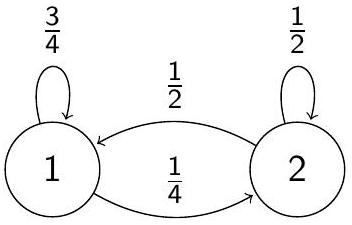
\includegraphics[max width=\textwidth, center]{2025_05_11_84d245f69223a25e0522g-40}

\begin{itemize}
  \item $J=\{1,2\}($ Hot $=1$, Cold=2)
  \item Transition matrix:
\end{itemize}

$$
R=\left[\begin{array}{ll}
\frac{3}{4} & \frac{1}{4} \\
\frac{1}{2} & \frac{1}{2}
\end{array}\right]
$$

Some possible sample paths $X_{0}, X_{1}, X_{2}, \ldots$ include:

$$
\begin{aligned}
& 2,2,1,1,2,1,1,2,2, \ldots \\
& 1,2,2,2,2,2,2,2,1, \ldots \\
& 1,2,1,2,1,2,1,2,1, \ldots
\end{aligned}
$$

How do we compute $P\left(X_{2}=1\right)$ ?

\section*{Transient analysis of a DTMC}
From a given state $i$, the next state is chosen with probability

$$
P\left(X_{n+1}=j \mid X_{n}=i\right)=P\left(X_{1}=j \mid X_{0}=i\right)=(R)_{i j}=r_{i j}
$$

Similarly, if we consider 2-step probabilities

$$
\begin{aligned}
P\left(X_{n+2}=j \mid X_{n}=i\right) & =\sum_{k \in J} P\left(X_{n+2}=j \mid X_{n+1}=k\right) P\left(X_{n+1}=k \mid X_{n}=i\right) \\
& =\sum_{k \in J} r_{i k} r_{k j}=\left(R^{2}\right)_{i j}
\end{aligned}
$$

A proof by induction can then be used to show that in general

$$
P\left(X_{n}=j \mid X_{0}=i\right)=\left(R^{n}\right)_{i j}
$$

that is element $(i, j)$ in the $n$th power of matrix $R$.

\section*{Transient analysis of a DTMC}
Therefore, by the Law of Total Probability

$$
\begin{aligned}
P\left(X_{n}=j\right) & =\sum_{i \in J} P\left(X_{n}=j \mid X_{0}=i\right) P\left(X_{0}=i\right) \\
& =\sum_{i \in J} P\left(X_{0}=i\right) P\left(X_{n}=j \mid X_{0}=i\right) \\
& =\sum_{i \in J} \pi_{0 i}\left(R^{n}\right)_{i j} \\
& =\left(\pi_{0} R^{n}\right)_{j}
\end{aligned}
$$

i.e. the $j$-th element of vector $\pi_{0} R^{n}$ gives us $P\left(X_{n}=j\right)$.

\section*{Example: modelling climate (continued)}
\begin{itemize}
  \item If today is cold ( $\pi_{02}=1$ ), will it be hot in two days from now?
\end{itemize}

$$
\pi_{0} R^{2}=\left[\begin{array}{ll}
0 & 1
\end{array}\right]\left[\begin{array}{ll}
0.688 & 0.312 \\
0.625 & 0.375
\end{array}\right]=[\underbrace{0.625}_{P\left(X_{2}=1\right)} 0.375]
$$

\begin{itemize}
  \item What is the long-term probability of hot and cold days?\\
$\lim _{n \rightarrow+\infty} \pi_{0} R^{n}=\left[\begin{array}{ll}\pi_{01} & \pi_{02}\end{array}\right]\left[\begin{array}{ll}0.667 & 0.333 \\ 0.667 & 0.333\end{array}\right]=[2 / 3,1 / 3]=\pi_{\infty}$\\
which holds in this example for any choice of vector $\pi_{0}$.
\end{itemize}

\section*{Long-term behaviour of a DTMC}
While transient analysis evaluates the detailed dynamics of the DTMC, we may alternatively look at situations where the DTMC stabilizes in some sense.

Two characterizations are the most common:

\begin{itemize}
  \item Limiting distribution: a vector $\pi_{\infty}$ such that
\end{itemize}

$$
\pi_{\infty}=\lim _{n \rightarrow+\infty} \pi_{0} R^{n}
$$

\begin{itemize}
  \item Steady-state (or stationary) distribution: a vector $\pi_{\infty}^{*}$ that is invariant under the DTMC transition matrix $R$. Namely:
\end{itemize}

$$
P\left(X_{n}=j\right)=\pi_{\infty, j}^{*}, \quad \forall n \geq 0, \forall j \in J .
$$

\section*{Existence and equivalence}
\begin{itemize}
  \item A limiting distribution, when it exists, is always a steady-state distribution, but the converse is not true.
  \item For example, starting the DTMC with $\pi_{0}=(1,0)$
\end{itemize}

$$
\begin{aligned}
R= & \left(\begin{array}{ll}
0 & 1 \\
1 & 0
\end{array}\right) \\
\pi_{1}= & (0,1) \\
\pi_{2}= & (1,0) \\
\vdots & \vdots \\
\pi_{2 n}= & (1,0) \\
\pi_{2 n+1}= & (0,1)
\end{aligned}
$$

therefore $\pi_{\infty}$ does not exist. However, $\pi_{\infty}^{*}=(0.5,0.5)$.

\section*{Uniqueness}
\begin{itemize}
  \item Are limiting and steady-state distributions unique?
  \item Not always, e.g., consider the following DTMC
\end{itemize}

$$
R=\left(\begin{array}{cccc}
0 & 0.5 & 0 & 0.5 \\
0 & 0.5 & 0.5 & 0 \\
0 & 0.5 & 0.5 & 0 \\
0 & 0 & 0 & 1.0
\end{array}\right)
$$

The limiting distribution exists but it is not unique, e.g.,

$$
\begin{aligned}
& \pi_{0}=(0,1,0,0) \quad \Rightarrow \pi_{\infty}=(0,0.5,0.5,0) \\
& \pi_{0}=(0,0,0,1) \quad \Rightarrow \pi_{\infty}=(0,0,0,1) \\
& \pi_{0}=(1,0,0,0) \quad \Rightarrow \pi_{\infty}=(0,0.25,0.25,0.5)
\end{aligned}
$$

\begin{itemize}
  \item All three $\pi_{\infty}$ in the above example are also valid steady-state distributions, thus $\pi_{\infty}^{*}$ is also not unique in general.
\end{itemize}

\section*{Classification of DTMCs}
When can we guarantee existence and uniqueness?

\begin{itemize}
  \item A DTMC is said to be irreducible if the directed graph associated to $R$ is strongly connected. This means that, for any pair $(i, j)$, there exist some sample path where, starting in state $i$, the DTMC eventually reaches state $j$.
  \item A DTMC is periodic if the time to return to a state is an integer multiple of a fixed period. Otherwise it is aperiodic.
  \item Q: are these DTMCs irreducible and aperiodic?
\end{itemize}

$$
R_{1}=\left(\begin{array}{ccc}
\frac{1}{3} & \frac{1}{3} & \frac{1}{3} \\
\frac{1}{4} & \frac{3}{4} & 0 \\
0 & 0 & 1
\end{array}\right) \quad R_{2}=\left(\begin{array}{ccc}
0 & 1 & 0 \\
0 & 0 & 1 \\
1 & 0 & 0
\end{array}\right) \quad R_{3}=\left(\begin{array}{ccc}
\frac{1}{3} & \frac{1}{3} & \frac{1}{3} \\
\frac{1}{2} & 0 & \frac{1}{2} \\
\frac{1}{4} & \frac{1}{4} & \frac{1}{2}
\end{array}\right)
$$

\section*{Uniqueness and existence conditions}
If a DTMC is irreducible and aperiodic, then:

\begin{itemize}
  \item Limiting and steady-state distributions both exist. They are also unique and identical to each other, i.e., $\pi_{\infty}=\pi_{\infty}^{*}$.
  \item The elements of $\pi_{\infty}$ are all strictly positive.
  \item $\pi_{\infty}$ is the solution of $\pi_{\infty} R=\pi_{\infty}$ subject to $\sum_{j} \pi_{\infty, j}=1$.
\end{itemize}

Without aperiodicity, an irreducible DTMC has no longer a valid limiting distribution $\pi_{\infty}$. However, the steady-state distribution $\pi_{\infty}^{*}$ exists also in this case and it is the unique positive solution of $\pi_{\infty}^{*} R=\pi_{\infty}^{*}$ subject to $\sum_{j} \pi_{\infty, j}^{*}=1$.

\section*{Example: climate modelling revisited}
The daily temperatures DTMC is irreducible and aperiodic with

$$
\pi_{\infty}=\pi_{0} \lim _{n \rightarrow \infty} R^{n}=(2 / 3,1 / 3)
$$

To see that $\sum_{j} \pi_{\infty, j}=1$ is necessary, note that\\
$\pi_{\infty}\left[\begin{array}{cc}3 / 4 & 1 / 4 \\ 1 / 2 & 1 / 2\end{array}\right]=\pi_{\infty} \Rightarrow \pi_{\infty}\left[\begin{array}{cc}-1 / 4 & 1 / 4 \\ 1 / 2 & -1 / 2\end{array}\right]=(0,0)$ (singular)\\
Now, replacing an equation with $\sum_{j} \pi_{\infty, j}=1$ we get instead

$$
\pi_{\infty}\left[\begin{array}{cc}
-1 / 4 & 1 \\
1 / 2 & 1
\end{array}\right]=(0,1) \Rightarrow \pi_{\infty}=(2 / 3,1 / 3)
$$

Moreover, it is also $\pi_{\infty}^{*}=\pi_{\infty}=(2 / 3,1 / 3)$.


\end{document}